\documentclass{exercise}
\usepackage{global-settings}
\usepackage{multicol}
\usepackage{subcaption}
\usepackage[version=4]{mhchem}

\usepackage{tikz}
\usepackage{tikz-feynman} % For Feynman diagrams

\def\modelsolution{1}

\setcounter{tutorial}{8}
\setcounter{exercise}{1}
\release{Mittwoch, 04.12.2024}
\submission{Mittwoch, 11.12.2024, 14 Uhr}


\DeclareMathOperator\artanh{artanh}

\begin{document}

\clearpage
\makeheader

\exercise{Fragen (2P)}
Stellen Sie \emph{pro Person} zwei relevante Fragen zu den Inhalten der Vorlesung \enquote{Einf\"uhrung in die Kern- und Elementarteilchenphysik}.

\exercise{Lorentztransformationen (7P)}

Die Lorentzgruppe ist die Gruppe an Transformationen auf Vierervektoren, unter denen die Minkowskimetrik (die Metrik des flachen Raumes) invariant bleibt:
\begin{equation}
    L := O(3,1) =  \left\{ \Lambda \in \mathbb{R}^{4 \times 4} \, | \, \Lambda_{\phantom{\mu} \mu}^\alpha \, g_{\alpha \beta} \, \Lambda_{\phantom{\nu} \nu}^\beta   = g_{\mu \nu} \right\} \,.
\end{equation} 

Eine wichtige Untergruppe der Lorentztransformationen (LTs) sind die eigentlich-orthochronen Lorentztransformationen
\begin{equation}
    L_+^\uparrow := \left\{ \Lambda \in L \, | \, \det \Lambda = 1 \, \wedge \, \text{sgn} \Lambda^0_{\phantom{0} 0} = 1 \right\} \,,
\end{equation} 
die ausschließlich Boosts und Rotationen umfasst.
Neben den eigentlich-orthochronen LTs existieren drei weitere Komponenten, die zusammen die Lorentzgruppe bilden.
Diese sind über Parit\"at und/oder Zeitumkehr mit der Untergruppe der eigentlich-orthochronen LTs verbunden.

\begin{enumerate}
    \item Geben Sie die Matrixformen der Paritäts- und Zeitumkehrtransformationen $P$ und $T$ an.
    
    \solution{
    \begin{align*}
        P &= \begin{pmatrix}
            1 & 0 & 0 & 0 \\
            0 & -1 & 0 & 0 \\
            0 & 0 & -1 & 0 \\
            0 & 0 & 0 & -1
        \end{pmatrix}
    \end{align*}
    \begin{align*}
        T &= \begin{pmatrix}
            -1 & 0 & 0 & 0 \\
            0 & 1 & 0 & 0 \\
            0 & 0 & 1 & 0 \\
            0 & 0 & 0 & 1
        \end{pmatrix}
    \end{align*}
    \textit{1 Punkt}
    }

    \item Zeigen Sie, dass $\det \Lambda = \pm 1$ gilt. 
    \solution{
        Wir starten mit
        \begin{equation}
            \Lambda^T g \Lambda = g \,.
        \end{equation}
        Dann folgt
        \begin{align*}
            \det(\Lambda^T) \det(g) \det(\Lambda) &= \det(g) \\
            \det(\Lambda^T) \det(\Lambda) &= 1 \\
            \det(\Lambda)^2 &= 1 \\
            \det(\Lambda) &= \pm 1 \,.
        \end{align*}
        \textit{1 Punkt}
    }

    \item Betrachten Sie einen Lorentzboost in $x$-Richtung mit
    \begin{equation}
        \label{eq:BoostsMatrix}
        \Lambda = \begin{pmatrix}
            \gamma & -\beta \gamma & 0 & 0 \\
            -\beta \gamma & \gamma & 0 & 0 \\
            0 & 0 & 1 & 0 \\
            0 & 0 & 0 & 1
        \end{pmatrix}
    \end{equation}
    und dem bekannten $\gamma = 1/\sqrt{1-\beta^2}$.
    Zeigen Sie, dass $\Lambda \in L_+^\uparrow$ gilt.

    \solution{
        Wir teilen den Beweis in drei Schritte auf:
        \begin{enumerate}
            \item  $\Lambda \in L$
            
            Offensichtlich ist $\Lambda$ eine reelle $4 \times 4$ da $\gamma \,, \beta \in \mathbb{R}$.
            Des Weiteren gilt:
            \begin{align*}
                \Lambda^T g \Lambda &= \begin{pmatrix}
                    \gamma & -\beta \gamma & 0 & 0 \\
                    -\beta \gamma & \gamma & 0 & 0 \\
                    0 & 0 & 1 & 0 \\
                    0 & 0 & 0 & 1
                    \end{pmatrix}^T
                    \begin{pmatrix}
                    1 & 0 & 0 & 0 \\
                    0 & -1 & 0 & 0 \\
                    0 & 0 & -1 & 0 \\
                    0 & 0 & 0 & -1
                    \end{pmatrix}
                    \begin{pmatrix}
                    \gamma & -\beta \gamma & 0 & 0 \\
                    -\beta \gamma & \gamma & 0 & 0 \\
                    0 & 0 & 1 & 0 \\
                    0 & 0 & 0 & 1
                    \end{pmatrix} \\
                    &= \begin{pmatrix}
                    \gamma & +\beta \gamma & 0 & 0 \\
                    -\beta \gamma & -\gamma & 0 & 0 \\
                    0 & 0 & -1 & 0 \\
                    0 & 0 & 0 & -1
                    \end{pmatrix}
                    \begin{pmatrix}
                    \gamma & -\beta \gamma & 0 & 0 \\
                    -\beta \gamma & \gamma & 0 & 0 \\
                    0 & 0 & 1 & 0 \\
                    0 & 0 & 0 & 1  
                    \end{pmatrix} \\
                    &= \begin{pmatrix}
                    1 & 0 & 0 & 0 \\
                    0 & -1 & 0 & 0 \\
                    0 & 0 & -1 & 0 \\
                    0 & 0 & 0 & -1
                    \end{pmatrix} = g \, 
            \end{align*}
            wobei wir $\gamma^2 = 1 - \beta^2$ nutzen.

            \item  $\text{sgn} \Lambda^0_{\phantom{0} 0} = 1$

            Das stimmt offensichtlich, weil $\Lambda^0_{\phantom{0} 0} = \gamma > 0$ immer gilt.

            \item  $\det \Lambda = 1$ 
            \begin{align*}
                \det \Lambda &= \det \begin{pmatrix}
                    \gamma & -\beta \gamma & 0 & 0 \\
                    -\beta \gamma & \gamma & 0 & 0 \\
                    0 & 0 & 1 & 0 \\
                    0 & 0 & 0 & 1 \\
                \end{pmatrix} \\
                &= 1 \cdot \begin{vmatrix}
                    \gamma & -\beta \gamma & 0 \\
                    -\beta \gamma & \gamma & 0 \\
                    0 & 0 & 1 \\
                    \end{vmatrix} \\
                &= \gamma^2 - \beta^2 \gamma^2 = 1 \,.
            \end{align*}
        \end{enumerate}
        \textit{2 Punkte}
    }
    \item Drücken Sie \eqref{eq:BoostsMatrix} durch die Rapidität $\eta = \artanh\left(\beta\right)$ aus. Welchen Vorteil kann es haben, mit $\eta$ zu rechnen?
    \solution{Ein möglicher Weg wäre: 
        \begin{align*}
            \beta           &= \tanh(\eta)\\
            \gamma          &= \dfrac{1}{\sqrt{1 - \tanh^2(\eta)}}\\
                            &= \dfrac{1}{\sqrt{ \dfrac{\cosh^2(\eta)}{\cosh^2(\eta)} - \dfrac{\sinh^2(\eta)}{\cosh^2(\eta)}}} \, \text{mit}\, \cosh^2(\eta) - \sinh^2(\eta) = 1\\
                            &= \cosh(\eta) \\
            \Rightarrow  \beta \gamma   &= \tanh(\eta)\cosh(\eta) = \sinh(\eta)
        \end{align*}
        Zusammen gilt:
        \begin{align*}
               \Lambda &= \begin{pmatrix}
                \cosh(\eta) & -\sinh(\eta) & 0 & 0 \\
                -\sinh(\eta) & \cosh(\eta) & 0 & 0 \\
                0 & 0 & 1 & 0 \\
                0 & 0 & 0 & 1 \\
            \end{pmatrix} \\
        \end{align*}
        Die Rapidität spannt den gesamten Wertebereich $\eta \in \left(-\infty, \infty\right)$, was intuitiver sein als $v \in \left(-c, c\right)$ kann.
        Außerdem ist $\eta$ additiv $\eta_\text{ges} = \eta_1 + \eta_2$\,.
        Es muss nicht die Formel für die relativistische Geschwindigkeitsaddition verwendet werden.\\
        \textit{1 Punkt}
        }
        \item Für einen kontravarianten Vektor $x^{\mu}$ gilt unter einer LT $x^{\mu} \rightarrow x'^{\mu} = \Lambda_{\phantom{\nu} \nu}^\mu x^{\nu}\,.$
        Bestimmen Sie das allgemeine Transformationsverhalten eines kovarianten Vektors $x_{\mu}$.
        \solution{
           $x_{\mu} \rightarrow x'_{\mu} = g_{\mu \nu} x'^{\nu} = g_{\mu \nu} \Lambda_{\phantom{\rho} \rho}^\nu x^{\rho} = \Lambda_{\mu \rho} x^{\rho} = \Lambda_{ \mu}^{\phantom{\nu} \nu} g_{\nu \rho} x^\rho = \Lambda_{ \mu}^{\phantom{\nu} \nu} x_\nu$ \\
           \textit{0,5 Punkte}
           }
        \item Bestimmen Sie das Transformationsverhalten der kovarianten Ableitung $\partial_\mu = \dfrac{\partial}{\partial x^\mu}$.\\
        \textit{Hinweis: Nutzen Sie, dass eine LT auch als $\dfrac{\partial x^\beta}{\partial x'^\alpha} = \Lambda^{\phantom{\beta} \beta}_\alpha$ geschrieben werden kann.}
        \solution{
            \begin{align}
                \dfrac{\partial}{\partial x^\mu} \rightarrow \dfrac{\partial}{\partial x'^\mu} = \dfrac{\partial x^\nu}{\partial x'^\mu}\dfrac{1}{\partial x^\nu} = \Lambda^{\phantom{\nu} \nu}_\mu \dfrac{1}{\partial x^\nu} = \Lambda^{\phantom{\nu} \nu}_\mu \partial_\nu\\
            \end{align}
            Die kovariante Ableitung transformiert wie eine kontravarianter Vektor.
            
            \textit{1 Punkt}
        }
        \item Zeigen Sie, dass eine Größe $x^\mu x_\mu$ tatsächlich invariant unter einer LT $x^\mu \rightarrow x'^\mu$ ist.
        \solution{
            \begin{align}
                x^\mu x_\mu = g_{\mu \nu} x^\mu x^\nu \rightarrow g_{\mu \nu} \Lambda_{\phantom{\rho} \rho}^\mu x^{\rho}  \Lambda_{\phantom{\sigma} \sigma}^\nu x^{\sigma} = \Lambda_{\phantom{\rho} \rho}^\mu g_{\mu \nu} \Lambda_{\phantom{\sigma} \sigma}^\nu  x^{\rho} x^{\sigma} = g_{\sigma \rho} x^{\rho} x^{\sigma} = x^{\rho} x_{\rho} = x^{\mu} x_{\mu}
            \end{align}
            \textit{0,5 Punkte}
        }

\end{enumerate}

\exercise{Gamma-Matrizen (4 Punkte)}

Sie haben Gamma-Matrizen bereits im Zuge der Dirac-Gleichung kennengelernt, wo sie eingesetzt wurden, um die verschiedenen Komponenten der Gleichung aneinander zu koppeln.
Diese $4 \times 4$-Matrizen treten, aber auch an anderer Stelle auf. 
So kann durch diese zum Beispiel ein konjugierter Spinor als $\bar{\psi} = \psi^\dagger \gamma^0$ geschrieben werden.
Ihr Verhalten wird durch den Antikommutator
\begin{equation}
    \label{eq:AntiKom}
    \left\{\gamma^\mu, \gamma^\nu \right\} = 2 g^{\mu \nu} \mathbb{1}_{4 \times 4}
\end{equation}
bestimmt.

Dabei ist $g^{\mu \nu}$ die Minkowskimetrik des flachen Raumes und $\gamma^\mu $ ein kontravarianter Vierervektor, in dessen Elemente die Gamma-Matrizen stehen.
Die Wahl der Gamma-Matrizen $\gamma^\mu$ ist nicht eindeutig.
Eine mögliche Wahl ist die sogenannte Dirac-Darstellung
\begin{align}
    \label{Gamma}
    \gamma^0 =   \begin{pmatrix}
                \mathbb{1}_{2 \times 2} & 0 \\
                0 & \text{-}\mathbb{1}_{2 \times 2} \\
    \end{pmatrix}\,, \qquad
    \gamma^\text{i} =   \begin{pmatrix}
        0 & \sigma^i \\
       \text{-} \sigma^i & 0 \\
    \end{pmatrix}
\end{align} 
mit $i = 1, 2, 3$ und den $2\times2$ Pauli-Matrixen $\sigma^i$.
\begin{enumerate}
    \item Zeigen Sie durch eine explizite Rechnung, dass die Gamma-Matrizen \eqref{eq:AntiKom} erfüllen.
    \solution{
    Eine Fallunterscheidung
    \begin{enumerate}
        \item $\mu = \nu = 0$
        \begin{align}    
            \left\{ \gamma^0, \gamma^0\right\} = 2 
            \begin{pmatrix}
            \mathbb{1} & 0 \\
            0       & \text{-}\mathbb{1} \\
            \end{pmatrix}
            \begin{pmatrix}
                \mathbb{1} & 0 \\
                0       & \text{-}\mathbb{1} \\
            \end{pmatrix}  
            = 2 
            \begin{pmatrix}
                \mathbb{1} & 0 \\
                0       & \mathbb{1} \\
            \end{pmatrix}  
        \end{align}
        \item $\mu = 0, \nu = i$
        \begin{align}
            \left\{ \gamma^0, \gamma^i\right\} &=
            \begin{pmatrix}
            \mathbb{1} & 0 \\
            0       & \text{-}\mathbb{1} \\
            \end{pmatrix}
            \begin{pmatrix}
                0 & \sigma^i \\
                -\text{-}\sigma^i & 0 \\
            \end{pmatrix} 
            +
            \begin{pmatrix}
                0 & \sigma^i \\
                -\text{-}\sigma^i & 0 \\
            \end{pmatrix} 
            \begin{pmatrix}
                \mathbb{1} & 0 \\
                0       & \text{-}\mathbb{1} \\
            \end{pmatrix}
            &=    \begin{pmatrix}
                0 & \sigma^i \\
                \sigma^i & 0 \\
            \end{pmatrix}
            +
            \begin{pmatrix}
                0 & \text{-}\sigma^i \\
                \text{-}\sigma^i & 0 \\
            \end{pmatrix} = 0
        \end{align}
        \item $\mu = i, \nu = j$
        \begin{align}
            \left\{ \gamma^i, \gamma^j\right\} &= \begin{pmatrix}
                0 & \sigma^i \\
                \text{-}\sigma^i & 0 \\
            \end{pmatrix}
            \begin{pmatrix}
                0 & \sigma^j \\
                \text{-}\sigma^j & 0 \\
            \end{pmatrix} +
            \begin{pmatrix}
                0 & \sigma^j \\
                \text{-}\sigma^j & 0 \\
            \end{pmatrix}
            \begin{pmatrix}
                0 & \sigma^i \\
                \text{-}\sigma^i & 0 \\
            \end{pmatrix}\\
             &= \begin{pmatrix}
                -\sigma^i \sigma^j& 0 \\
                0 & -\sigma^i \sigma^j \\
            \end{pmatrix} +
            \begin{pmatrix}
                -\sigma^j \sigma^j& 0 \\
                0 & -\sigma^j \sigma^i \\
            \end{pmatrix}\\
              &= \begin{pmatrix}
                \text{-} \left\{ \sigma^i, \sigma^i \right\}& 0 \\
                0 & \text{-}\left\{ \sigma^i, \sigma^i \right\} \\
            \end{pmatrix} = \text{-}2 \delta_{ij}
            \begin{pmatrix}
                \mathbb{1} 0 \\
                0 & \mathbb{1} \\
            \end{pmatrix} = 2 g_{ij} \mathbb{1}_{4 \times 4}
         \end{align}
        \end{enumerate}
        \textit{2 Punkte}}
         \item Zeigen Sie ohne explizites Einsetzen $\gamma^\mu \gamma_\mu = 4 \cdot \mathbb{1}_{4 \times 4}$ und $\gamma^\mu \gamma^\nu \gamma_\mu = \text{-} 2 \gamma^\nu $.
         \solution{
            \begin{align*}
                \gamma^\mu \gamma_\mu &= g_{\mu \nu} \gamma^\mu \gamma^\nu \\
                &= \frac{1}{2} \left( g_{\mu \nu} \gamma^\mu \gamma^\nu + g_{\mu \nu} \gamma^\mu \gamma^\nu \right) 
                \quad &\text{ (Benenne um } \mu \rightarrow \nu \text{ im rechten Term)} \\
                &= \frac{1}{2} \left( g_{\mu \nu} \gamma^\mu \gamma^\nu + g_{\nu \mu} \gamma^\nu \gamma^\mu \right) \\
                &= \frac{1}{2} \left( g_{\mu \nu} \gamma^\mu \gamma^\nu + g_{\mu \nu} \gamma^\nu \gamma^\mu \right) \\
                &= \frac{1}{2} g_{\mu \nu} \cdot 2 g^{\mu \nu} \, 1_{4 \times 4} \\
                &= g_{\mu \nu} g^{\mu \nu} \, 1_{4 \times 4} = 4 \cdot 1_{4 \times 4}.
            \end{align*}
            \begin{align*}
                \gamma^\mu \gamma^\nu \gamma_\mu &= \gamma^\mu \left( \gamma^\nu \gamma_\mu + \gamma_\mu \gamma^\nu - \gamma_\mu \gamma^\nu \right) \\
                &= \gamma^\mu \left( 2 \delta^\nu_\mu \cdot \mathbb{1}_{4 \times 4} - \gamma_\mu \gamma^\nu \right) 
                \quad &\text{(mit } \gamma^\mu \gamma_\mu = 4 \cdot \mathbb{1}_{4 \times 4}\text{)} \\
                &= 2 \gamma^\nu \cdot \mathbb{1}_{4 \times 4} - 4 \gamma^\nu \cdot \mathbb{1}_{4 \times 4} \\
                &= -2 \gamma^\mu \cdot \mathbb{1}_{4 \times 4}.
            \end{align*}
            \textit{1 Punkt}
            }
            \item Zeigen Sie zusätzlich $(\gamma^\mu)^\dagger = \gamma^0 \gamma^\mu \gamma^0$.
            \solution{
                Da $\gamma^0$ reell und symmetrisch ist, gilt offensichtlich $(\gamma^0)^\dagger = \gamma^0$ \\
                $\gamma^i$ ist entweder antisymmetrisch oder imaginär $(\gamma^i)^\dagger = \text{-}\gamma^i$\\
                \begin{align}
                    (\gamma^0)^\dagger &= \gamma^0 \gamma^0 \gamma^0 \quad \text{und}\\
                    (\gamma^i)^\dagger &= \text{-}\gamma^i = - \gamma^i \gamma^0 \gamma^0 = \gamma^0 \gamma^i \gamma^0 \,.
                \end{align}
                \textit{0,5 Punkte}}
            \item Es kann eine weitere Gamma-Matrix $\gamma^5 = i \gamma^0 \gamma^1 \gamma^2 \gamma^3$ definiert werden.\\
            Zeigen Sie, dass $\left\{\gamma^\mu, \gamma^5\right\} = 0$ gilt.
            \solution{
                \begin{align*}
                     \gamma^0 \gamma^5 &= i \gamma^0 \gamma^0 \gamma^1 \gamma^2 \gamma^3 
                    = -i \gamma^0 \gamma^1 \gamma^2 \gamma^3 \gamma^0 = -\gamma^5 \gamma^0. \\
                     \gamma^i \gamma^5 &= i \gamma^i \gamma^0 \gamma^1 \gamma^2 \gamma^3 = i  \gamma^0 \gamma^1 \gamma^2 \gamma^3 \gamma^i 
                    = -\gamma^5 \gamma^i \quad \text{(mit } i = 1, 2, 3) 
                \end{align*}
                \textit{0,5 Punkte}}
\end{enumerate}

section{Schwache Wechselwirkung (10P)}

\begin{enumerate}
    \item Erklären Sie was die V-A Struktur der schwachen Wechselwirkung beschreibt.
    \solution{Vektor - Aktialvektor bedeuted, dass die schwache WW nur an linkshändigen Teilchen koppelt. Mathematische ist $1 - \gamma^5$ linkshändige Prjektor, der dazu führt. dass Parität maximal gebrochen wird.}

    \item Der Übergang $\Gamma_{i \to f}$ von einem Anfangszustand zu einem Endzustand kann durch Fermis Goldene Regel beschrieben werden.
    Geben Sie diese an und beschreiben Sie ihre Komponenten.
    \solution{
        $\Gamma_{i \to f} = \dfrac{2\pi}{\hbar} \left| M_{f,i}\right|^2 \mathrm{d} \Pi_\text{LIPS}$ Das Matrixelement $M_{f,i}$ beschreibt die Amplitude des Übergang und  $\mathrm{d} \Pi_\text{LIPS}$ beschreibt die Anzahl der möglichen Endzustände.
    }
    \item Zeichen Sie das Feynman-Diagramm, welches den Zerfall des $\mu^-$ auf Tree-Level beschreibt.
    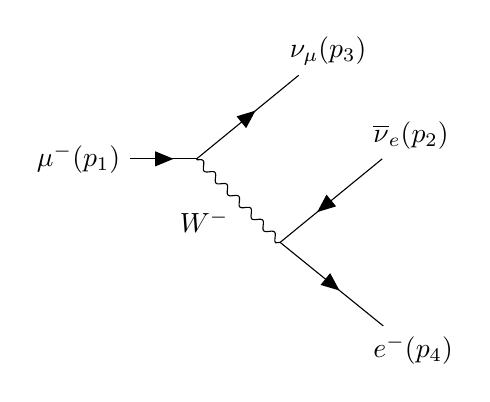
\begin{tikzpicture}
        \begin{feynman}
          \vertex (a) {\(\mu^{-}(p_1)\)};
          \vertex [right=of a] (b);
          \vertex [above right=of b] (f1) {\(\nu_{\mu}(p_3)\)};
          \vertex [below right=of b] (c);
          \vertex [above right=of c] (f2) {\(\overline \nu_{e}(p_2)\)};
          \vertex [below right=of c] (f3) {\(e^{-}(p_4)\)};
      
          \diagram* {
            (a) -- [fermion] (b) -- [fermion] (f1),
            (b) -- [boson, edge label'=\(W^{-}\)] (c),
            (c) -- [anti fermion] (f2),
            (c) -- [fermion] (f3),
          };
        \end{feynman}
      \end{tikzpicture}
    \item Wenden Sie die Feynman-Regel an, um das Matrixelement $M$ zu bestimmen.\\
    \textit{Hinweis: Eine explizite Berechnung von $M$ ist nicht notwendig.} 
    \solution{
        $M = \dfrac{g_\text{w}^2}{8\left(M_\text{W} c \right)^2} \left[\overline{u}(p_3) \gamma^\mu \left( 1 - \gamma^5\right) u\left( p_1\right)\right]  \left[\overline{u}(p_4) \gamma_\mu \left( 1 - \gamma^5\right) v\left( p_2\right)\right]$
    }

    Die Zerfallsrate in Abhängigkeit der Elektronenenergie ist gegeben durch 
    \begin{equation}
        \dfrac{\mathrm{d} \Gamma}{\mathrm{d} E_\text{e}} = \left(\dfrac{g_\text{w}}{M_\text{W}c}\right)^4 \cdot \left(1 - \dfrac{4 E_e}{3 m_\mu c²}\right) \,.
    \end{equation}
    \item Bestimmen Sie die totale Zerfallsrate und geben sie eine Gleichung für die Lebenszeit eines $\mu^-$.
    \solution{
        \begin{align}
            \Gamma =& \left(\dfrac{g_\text{w}}{M_\text{W}c}\right)^4 \dfrac{m_\mu^2}{2\hbar \left( 8 \pi\right)^3}
            \int_{0}^{1/2 m_\mu c^2} E^2\left( 1 - \dfrac{4E}{3m_\mu c^2}\right) \, \mathrm{d}E \\
                =& \left(\dfrac{m_\mu g_\text{w}}{M_\text{W}}\right)^4 \dfrac{m_\mu c^2}{12 \hbar \left(8 \pi \right)^3}
        \end{align}
        Für die Lebenszeit gilt $\tau = \dfrac{1}{\Gamma}$\,.
    }

    \item Vergleichen Sie das Ergebnis mit dem Literaturwert. Erklären Sie mögliche Abweichungen.
    \solution{
        Es entstehen Abweichungen, weil hier nur Tree-Level Diagramme betrachtet werden.
    }
    \item Welcher der beiden Zerfälle $\pi^- \to e^- \bar{\nu}_{\text{e}}$ und $\pi^- \to \mu^- \bar{\nu}_{\mu}$ tritt häufiger auf? Begründen Sie.
    \solution{Der erste Zerfall tritt seltener auf, da dieser Helizitätsunterdrückt ist.}

    \item Betrachten Sie nun den Prozess $e^+ e^- \to \mu^+ \mu^-$ auf Tree-Level. Zeichen Sie alle möglichen Diagramme. Bei welchen Energien tritt dieser Prozess besonders häufig auf? 
    \solution{
        s-Kanal der elektromagnetischen WW und s-Kanal über das $Z^0$.
        Besonders häufig bei niedrigen Energien über die elektromagnetische WW und am $Z^0$ Pol.
    }
\end{enumerate}


\section{Starke Wechselwirkung (10P)}

\begin{enumerate}
\item An welche Ladung koppelt die starke Wechselwirkung? Wie kann man sie messen?%Exam 22/23
\solution{
    Sie koppelt an die Farbladung. Da messbare Zustände immer farbneutral sind, lässt sich die Farbladung nicht messen.%Exam 22/23
}
\item Was wird durch asymptotische Freiheit und Confinement in Bezug auf die starke Wechselwirkung beschrieben?%Exam 22/23
\solution{Asymptotische Freiheit und Confinement beschreiben das Verhalten der Kopplungskonstante der starken Wechselwirkung. Im Niedrig-Energie-Limes ist diese sehr groß, während sie für große Energieskalen sich asymptotisch null nähert.}
\end{enumerate}
Das Quark-Parton-Modell erlaubt es, tiefinelastische Streuung von Leptonen an Nukleonen bei hohen Impulsüberträgen anschaulich zu deuten.
\begin{enumerate}

\item Was sind Partonen? Warum kann in der tiefinelastischen Streuung angenommen werden, dass Streuung an Partonen elastisch stattfindet? Zeichnen sie dazu eine Skizze.
\solution{ Partonen wurden eingeführt, um die Substruktur von Hadronen zu beschreiben. Sie sind heute mit Quarks und Gluonen identifizierbar. Partonen werden als punktförmig angenommen, sodass elastische Streuung möglich ist.}

\item Was passiert, wenn Sie zu niedrigeren Elektron-Energien übergehen?
\solution{
    tiefinelastische Streuung kann nicht mehr stattfinden, wir erwarten dann inelastische Streuprozesse, und bei noch niedrigeren Energien elastische e-p Streuung
}
\item Gluonen sind masselose Austauschteilchen. Photonen sind ebenfalls masselos. Könnte es sich also bei Photonen um das neunte farblose Gluon handeln  %Griffiths
\item Schätzen Sie das Verzweigungsverhältnisse $\frac{\text{BR}(B^0 \to \pi^+ \pi^-)}{\text{BR}(B^0 \to \pi^0 \pi^0)}$ ab.%Exam 20/21 Nr.4 d2)
\solution{Es wird $\frac{\text{BR}(B^0 \to \pi^+ \pi^-)}{\text{BR}(B^0 \to \pi^0 \pi^0)} \approx 3$ erwartet, da bei $\text{BR}(B^0 \to \pi^0 \pi^0)$ alle vier Quarks die gleich Farbladung tragen müssen.
    \begin{tikzpicture}
        \begin{feynman}
            \vertex (a) {\(B^0 (d\bar{b})\)};
            \vertex [right=2cm of a] (b);
            \vertex [above right=1.5cm and 2cm of b] (f1) {\(\pi^+ (u\bar{d})\)};
            \vertex [below right=1.5cm and 2cm of b] (f2) {\(\pi^- (d\bar{u})\)};
            
            \diagram*{
                (a) -- [fermion] (b) -- [fermion] (f1),
                (b) -- [anti fermion] (f2),
                (b) -- [boson, edge label=\(W^-\)] (f2),
            };
            
        \end{feynman}
    \end{tikzpicture}
            \begin{tikzpicture}
                \begin{feynman}
                    \vertex (a) {\(B^0 (d\bar{b})\)};
                    \vertex [right=2cm of a] (b);
                    \vertex [above right=1.5cm and 2cm of b] (f1) {\(\pi^0 (u\bar{u})\)};
                    \vertex [below right=1.5cm and 2cm of b] (f2) {\(\pi^0 (d\bar{d})\)};
                    
                    \diagram*{
            (a) -- [fermion] (b) -- [fermion] (f1),
            (b) -- [anti fermion] (f2),
            (b) -- [boson, edge label=\(W^-\)] (f2),
            };
        \end{feynman}
    \end{tikzpicture}
}
        
\end{enumerate}

\end{document}